% Corregir redacción, plural y presente
  
% TODO
% - Arquitectura sistemas NLG (3 slides aprox)
% - Requerimientos. Aca presentar la clase de prueba generada por Fastest y comentar algunas de las tranformaciones que le tendremos que hacer para generar mejores descripciones.
% - Desarrollo, ya con todos los requerimientos presentados, deberían ser unas pocas slides (3 o 4) por etapa.
%
% 0) Hacer algo con los exampleblock (o usarlos para todos los esquemas Z o no usarlo para ninguno). En caso de usarlos, ver la forma que queden más "lindos", que no ocupen el 100% de la página en una lista de items por ej. Multiple columns para clase y caso de prueba del ejemplo?
% 1) Armar un bosquejo de las slides que faltan y luego pegarle una corregida agregando todas las notas necesarias.
%
  
% Copyright 2004 by Till Tantau <tantau@users.sourceforge.net>.
%
% In principle, this file can be redistributed and/or modified under
% the terms of the GNU Public License, version 2.
%
% However, this file is supposed to be a template to be modified
% for your own needs. For this reason, if you use this file as a
% template and not specifically distribute it as part of a another
% package/program, I grant the extra permission to freely copy and
% modify this file as you see fit and even to delete this copyright
% notice. 
  
\documentclass[pdf]{beamer}
\usepackage[spanish]{babel}
\usepackage[utf8]{inputenc}
\usepackage{czt}
\usepackage[]{algorithm}
\usepackage{algpseudocode}

\usepackage{minted}
\usepackage{xcolor}

\usepackage[most]{tcolorbox}

%\usetheme{Madrid}
%\usetheme{Antibes}
\usetheme{Copenhagen}
\mode<presentation>{} 

\AtBeginSection[]
{
  \begin{frame}<beamer>
    \frametitle{Contenidos}
    \tableofcontents[currentsection]
  \end{frame}
}
  
%\title{Generación de lenguaje natural a partir de clases de prueba del \textit{test template framework}}
  
% A subtitle is optional and this may be deleted
%\subtitle{Optional Subtitle}
  
%\author{F.~Author\inst{1} \and S.~Another\inst{2}}
% - Give the names in the same order as the appear in the paper.
% - Use the \inst{?} command only if the authors have different
%   affiliation.
  
%\institute[Universities of Somewhere and Elsewhere] % (optional, but mostly needed)
%{
%  \inst{1}%
%  Department of Computer Science\\
%  University of Somewhere
%  \and
%  \inst{2}%
%  Department of Theoretical Philosophy\\
%  University of Elsewhere}
% - Use the \inst command only if there are several affiliations.
% - Keep it simple, no one is interested in your street address.
  
%\date{Conference Name, 2013}
% - Either use conference name or its abbreviation.
% - Not really informative to the audience, more for people (including
%   yourself) who are reading the slides online
  
\subject{Computer Science}
% This is only inserted into the PDF information catalog. Can be left
% out. 
  
% If you have a file called "university-logo-filename.xxx", where xxx
% is a graphic format that can be processed by latex or pdflatex,
% resp., then you can add a logo as follows:
  
\pgfdeclareimage[height=0.5cm]{university-logo}{../img/unr.png}
\logo{\pgfuseimage{university-logo}}
  
% Delete this, if you do not want the table of contents to pop up at
% the beginning of each subsection:
%\AtBeginSubsection[]
%{
%    \begin{frame}<beamer>{Contenidos}
%        \tableofcontents[currentsection,currentsubsection]
%    \end{frame}
%}
  
% Let's get started
\begin{document}
  
\title[NLG a partir de clases de prueba del TTF]{Generación de lenguaje natural a partir de clases de prueba del \textit{test template framework}}
\institute[FCEIA - UNR]{
  Departamento de Ciencias de la Computación\\
  Facultad de Ciencias Exactas, Ingeniería y Agrimensura\\
  Universidad Nacional de Rosario
}
\author[Julian De Tomasi]{\begin{tabular}{r@{ }l} 
  Autor:      & Julian De Tomasi \\[1ex]
  Directores: & Maximiliano Cristiá\\
  & Brian Plüss
  \end{tabular}}
\date{Abril, 2016}
  
\begin{frame}
  \titlepage
\end{frame}
  
%\begin{frame}{Outline}
  %\tableofcontents
  % You might wish to add the option [pausesections]
%\end{frame}
  
\section{Introducción}
  
\begin{frame}{Motivación}{}
  \begin{itemize}
                          
    \note[item]{ Las metodologías de \emph{testing} basado en modelos parten de un modelo formal (o especificación) del software a testear y a partir del mismo son generados los casos de prueba.}
                                      
    \note[item]{ Es una de las técnicas de testing más prometedoras para la verificación de software crítico.}
                                      
    \note[item]{ El \emph{Test Template Framework} (TTF) es un caso particular del testing basado en modelos. Utiliza como modelo de entrada una especificación formal en notación Z y establece cómo generar \emph{casos de prueba} para las operaciones incluidas en la especificación.}
                                                  
    \note[item]{ El TTF propone en primera instancia obtener casos de prueba abstractos a partir de una especificación llamados \emph{clases de prueba} y luego, a partir de los mismos, generar los \emph{casos de prueba concretos}.}
                                                              
    \note[item]{ En estos casos, una descripción en lenguaje natural de cada caso de prueba debería acompañar a los mismos a fin de hacerlos accesibles para los expertos en el dominio.}
    
    \note[item]{ Usualmente también se realizan procesos independientes de validación y verificación, llevados a cabo por expertos en el dominio que generalmente no poseen conocimiento técnico para comprender lo que se esta siendo testeado.}
    
    \note[item]{En sistemas en los que hay una gran cantidad de casos de prueba, traducir manualmente los mismos podría introducir errores humanos, reduciendo la calidad de las descripciones además de incrementar el costo del testing.}
    
    \item El TTF (\emph{Test Template Framework}) nos permite generar casos para un sistema del cual se tiene una especificación formal en Z.
    
    \item Usualmente se realizan validaciones y verificaciones llevadas a cabo por expertos en el dominio que generalmente no poseen conocimiento técnico para comprender los casos de prueba resultado del TTF.
    
    \item Contar con una descripción en lenguaje natural de los casos de prueba resultaría de gran ayuda para estos procesos de validación y verificación.
                                                              
  \end{itemize}
\end{frame}
                                      
                                      
\begin{frame}{Ejemplo: TTF}{Especificación \emph{LookUpOk}}

    Utilizaremos la operación \emph{LookUpOk} (parte de la especificación para una tabla de símbolos) para ilustrar los resultados del TTF que luego serán entrada de nuestro sistema de NLG.
                                          
  \note[item]{
    Una tabla de símbolos es una estructura de datos utilizada por un compilador o intérprete durante el proceso de traducción de un lenguaje de programación donde cada símbolo en el código del programa (variables, constantes, funciones, etc.) se asocia con información como la ubicación, tipo de datos, \textit{scope} de variables, etc. En general, en una tabla de símbolos se realizan dos operaciones: inserción/actualización y búsqueda.
  }
                                          
  \vspace{-0.5cm}
  \begin{schema}{LookUpOk}
    \Xi ST \\
    s?: SYM \\
    v!: VAL \\
    rep!: REPORT
    \where
    s? \in \dom st \\
    v! = st~s? \\
    rep! = ok
  \end{schema}
                                          
  \note[item]{
    El tipo básico \emph{SYM} representará el conjunto de todos los símbolos aceptados por el compilador/interprete, mientras que \emph{VAL} abstraerá el conjunto de toda la información que pudiese estar asociada a un símbolo.
  }
                                          
  \note[item]{
    Finalmente, resulta natural pensar que la tabla de símbolos establece una relación funcional entre los símbolos aceptados y la información asociada a cada uno de ellos.
  }                                 
\end{frame}
                                      
\begin{frame}{Ejemplo: TTF}{Designaciones \emph{LookUp}}
                                            
  \note[item]{
    Vinculamos los términos del modelo formal a elementos relacionados con el dominio de aplicación mediante las designaciones.
  }
                                            
  \note[item]{
    Las designaciones sirven en primera instancia cuando se empieza a escribir la especificación para diferenciar un fenómeno en particular y darle un nombre. Luego, le será de utilidad al programador a la hora de leer la especificación.
  }
                                            
  \note[item]{
    Para nosotros las designaciones resultarán la principal fuente de conocimiento para nuestro sistema de NLG. Y serán fundamentales para que éste pueda generar descripciones independientes del dominio de aplicación.
  }
                                            
  \begin{itemize}                                            
    \item{
      Podemos tener las siguientes designaciones para el ejemplo anterior: \\
      \begin{minipage}{9cm}
        \begin{exampleblock}{}
        \vspace{-.5cm}
        \begin{align*} 
            & \text{Símbolo a actualizar}                      & \approx &~s?      \\
            & \text{Símbolos cargados en la tabla} & \approx &~\dom st 
        \end{align*}
      \end{exampleblock}
      \end{minipage}
    }
    
    \item Además del propósito habitual de las mismas, las designaciones resultan una fuente de conocimiento para nuestro sistema de NLG.
  \end{itemize}
                                            
  \note[item]{
    Los sistemas de generación de lenguaje natural generalmente utilizan un diccionario de palabras o frases, las cuales se utilizan para referirse a fenómenos del dominio. En nuestro caso, el dominio de aplicación dependerá de la especificación en cuestión y de lo que se modele con la misma, por lo tanto, las designaciones resultarán nuestra única fuente de textos dependientes del dominio y es por eso que serán un elemento fundamental para nuestro sistema de NLG.
  }
                                            
\end{frame}
                                      
\begin{frame}{Ejemplo: TTF}{Caso de prueba para \emph{LookUp}}

  \begin{itemize}
    \item{
      Podríamos intentar describir los casos de prueba generados por el TTF. \\
      \vspace{-.5cm}
      \begin{schema}{LookUp\_ SP\_ 1\_ TCASE}\\
        LookUp\_ SP\_ 1 
        \where
        st = \{ ( sym0 , val0 ) \} \\
        s? = sym0
      \end{schema}
    }
    
    \vspace{-.5cm}
    \item Pero nos estaríamos perdiendo de información valiosa contenida en las \textbf{clases de prueba}.
  \end{itemize}
\end{frame}
                                
\begin{frame}{Ejemplo: TTF}{Clase de prueba para \emph{LookUp}}
  \begin{itemize}
    \item{
      Las \textbf{clases de prueba} son las que contienen la información referente a las alternativas funcionales que se intentan testear mediante cada \emph{caso de prueba} generado.\\
      
    }
                                               
    \note[item]{
      La clase de prueba presentada es una versión simplificada de la generada por Fastest. Más adelante veremos la clase de prueba generada por la herramienta y como nuestro sistema trabajará con ella para obtener una similar a la anterior.
    }
  \end{itemize}
  
  \vspace{-0.8cm}
  \begin{schema}{LookUp\_ SP\_ 1}\\
    st : SYM \pfun VAL \\
    s? : SYM 
    \where
    s? \in \dom st \\
    \dom st = \{ s? \}
  \end{schema}
\end{frame}
                                      
\begin{frame}{Ejemplo: TTF}{Descripción para \emph{LookUp\_SP\_1}}
  \begin{itemize}
    \item  Descripción en lenguaje natural para \emph{LookUp\_SP\_1}:
  \end{itemize}
  
  \begin{tcolorbox}[colback=gray!5!white,colframe=gray!50!black,
  colbacktitle=gray!75!black,title=LookUp\_ SP\_ 1]
  Se intenta buscar el valor de un símbolo, cuando:
     \begin{itemize}
        \item[--]{El símbolo a buscar pertenece a los símbolos cargados en la tabla.}
        \item[--]{El símbolo a buscar es el único elemento de los símbolos cargados en la tabla.}
     \end{itemize}
  \end{tcolorbox}
\end{frame}

\begin{frame}{Generación de Lenguaje Natural}{}
\begin{columns}[t] % align columns
\begin{column}{.60\textwidth}
  \begin{itemize}
  
    \item Utilizamos la metodología propuesta por Reiter y Dale para la construcción de sistemas de NLG.

    \item Ésta propone un análisis de requerimientos en base a un corpus objetivo y una arquitectura de \emph{pipeline} conformada por tres etapas: \textbf{document planning}, \textbf{microplanning} y \textbf{surface realization}.

  \end{itemize}
\end{column}%
\hfill%
\begin{column}{.40\textwidth}
  \begin{figure}[H]
    \centering
    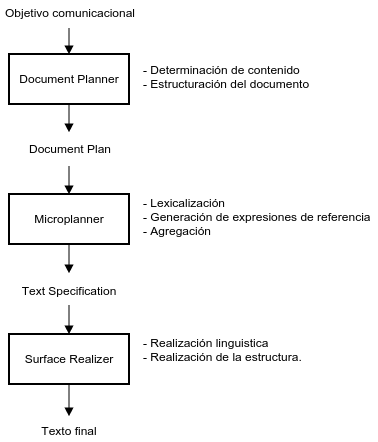
\includegraphics[scale=0.3]{img/arquitectura.png}
  \end{figure}
\end{column}%
\end{columns}
\end{frame}
                                
\begin{frame}{Objetivo general}{}
  \begin{itemize}
   
    \item Desarrollar un una solución para la generación automática de descripciones en lenguaje natural para los casos de prueba generados por el TTF.
    
    \vspace{0.4cm}
    \item Lograr una solución independiente del número de operaciones del modelo así como del dominio de aplicación del mismo. 
    
    \vspace{0.4cm}
    \item Para esto, utilizamos técnicas de generación de lenguaje natural, trabajando principalmente con las clases de prueba y haciendo uso de la información contenida en las designaciones. 
  
    %\item El objetivo de este trabajo, será entonces, desarrollar una solución para la generación automática de descripciones para los casos de prueba generados por el TTF. Para esto, utilizaremos técnicas de \emph{generación de lenguaje natural}.
    %\item Trabajaremos principalmente con las \emph{clases de prueba}, ya que estas son las que contienen la información referente a las alternativas funcionales que se intentan testear mediante cada \emph{caso de prueba}.
    %\item Pretendemos una solución independiente del número de operaciones del modelo así como del dominio de aplicación del mismo. Para esto, junto con la utilización de técnicas de NLG, haremos uso de la información contenida en las designaciones.
  \end{itemize}
\end{frame}
                                
\section{Requerimientos}
\begin{frame}{Corpus de descripciones}{Introducción}
  \begin{itemize}
    \item Reiter y Dale proponen la construcción de un \textbf{corpus} de ejemplos para extraer los requerimientos de un sistema NLG.
    \item Un corpus no es más que una colección de ejemplos de entrada y las respectivas salidas que se esperan del sistema de NLG. 
    \item Para construir el corpus que utilizamos en este trabajo, describimos manualmente un conjunto de clases de pruebas generadas con Fastest para distintas especificaciones. Buscamos cubrir todo el rango de textos que esperamos que nuestro sistema sea capaz de producir.
      %\item En base al corpus, se extrajeron requerimientos fundamentales que sustentan una gran parte de las decisiones presentadas a lo largo del trabajo.
  \end{itemize}
\end{frame}


\begin{frame}{Corpus}{Requerimientos más relevantes}
  Resultados más relevantes del análisis del corpus:
  \begin{itemize}
    \item Determinamos la estructura que deberán tener las descripciones de cada clase de prueba en el texto final.
    \item Se detectaron tareas de razonamiento con los datos, como la reducción de expresiones y eliminación de tautologías. 
    \item Se analizó la verbalización de expresiones y el rol de las designaciones en esta tarea. 
    \item Se determinaron aspectos gramaticales que nuestro sistema de NLG debió contemplar. 
  \end{itemize}
\end{frame}

\begin{frame}[fragile]{Verbalización de expresiones}{}
  \begin{itemize}
  \item{ Observamos del corpus patrones que se repiten en las descripciones, producto de los operadores de Z presentes en los predicados que se describen. Por ejemplo:

	\begin{enumerate}
	\item $s? \in \dom st$ $\rightarrow$ \emph{``El símbolo a buscar \textbf{pertenece a}  a los símbolos cargados en la tabla.''}
	\item $num? \in \dom cajas$ $\rightarrow$ \emph{``El número de cuenta del nuevo cliente \textbf{pertenece a} los números de cuenta cargados en el banco.''}
    \end{enumerate}

  }
  
  \item La verbalización de predicados es uno de los desafíos más importantes de este trabajo.
  
  \end{itemize}

\end{frame}

\begin{frame}[fragile]{Verbalización de expresiones}{Reglas de verbalización}

  A continuación mostramos, a modo de ejemplo, una regla de verbalización para operador $\in$:
  
  %\vspace{-0.8cm}
  %\begin{multline*}
  \begin{figure}[H]
  $\texttt{verb'} (x \in X) \rightarrow \texttt{verb}(x) + \text{\emph{``pertenece(n) a''}} + \texttt{verb}(X)$
  \end{figure}
  %\end{multline*}
  
  ¡Debemos considerar también los casos en los que la expresión a verbalizar se encuentre designada!
  
  \begin{figure}[H]
  \begin{minted}[escapeinside=@@]{haskell}
  verb (@$exp$@) = if esta_designada(@$exp$@)
               then designacion(@$exp$@)
               else verb'(@$exp$@)
  \end{minted}
  \end{figure}

  

\end{frame}
                                
\section{Desarrollo}
                                
\subsection{Document Planning}
                                
\begin{frame}{Document Planner}{}
  \begin{columns}[T] % align columns
  \begin{column}{.60\textwidth}

  \begin{itemize}
    \item Es el primer módulo del sistema NLG.
    \item Está encargado de que el documento final tenga toda la información requerida por el usuario y que la misma se encuentre estructurada de una forma relativamente coherente.
    \item Desarrolla las tareas de \textbf{determinación de contenido} y \textbf{estructuración del documento.}
  \end{itemize}  
  
  \end{column}%
  \hfill%
  \begin{column}{.40\textwidth}
  \begin{figure}[H]
    \centering
    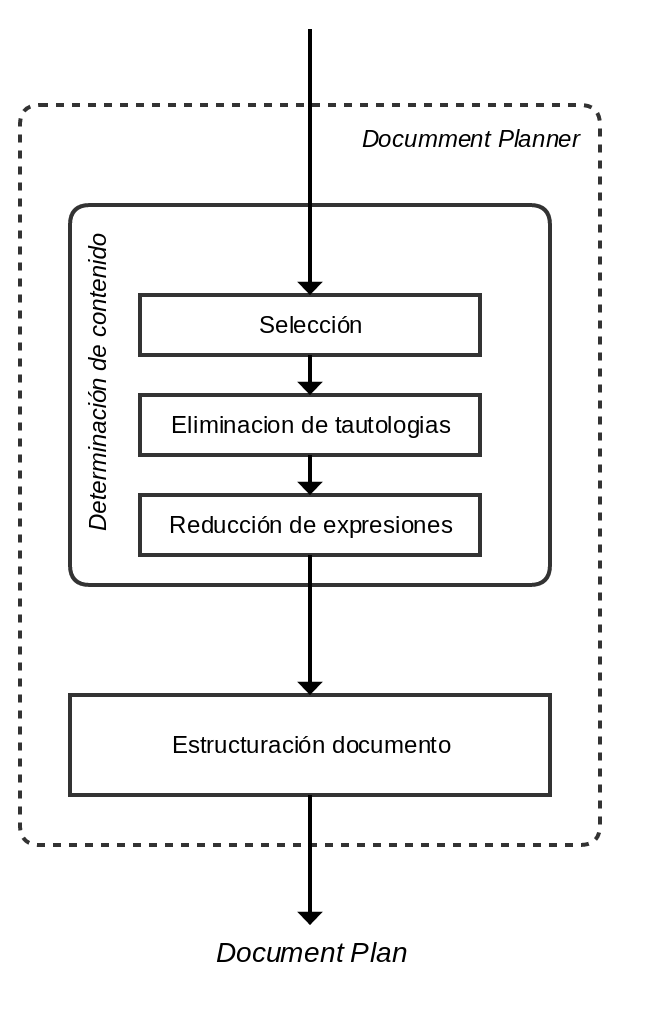
\includegraphics[scale=0.17]{img/tareas_document_planner.png}
  \end{figure}
  \end{column}%
  \end{columns}
  
  
  %\begin{itemize}
  %  \item Es el primer módulo del pipeline de nuestro sistema.
  %  \item Es el encargado de que el documento final tenga toda la información requerida por el usuario y que la misma se encuentre estructurada de una forma relativamente coherente.
  %  \item Este módulo será el ecargado de que se lleven a cabo las tareas de \textit{determinación de contenido} y \textit{estructuración del documento}
  %\end{itemize}
\end{frame}
                                
%\begin{frame}{Entrada y salida}{}
%    \begin{itemize}
%        \item TODO Imagen
%    \end{itemize}
%\end{frame}

\begin{frame}[fragile]{Document Planner}{Entrada y salida}
\begin{columns}[T] % align columns
\begin{column}{.50\textwidth}
  Entrada
  \rule{\linewidth}{1pt}
  
  \begin{itemize}
  \item Objetivo comunicacional.
  
  \item{Fuente de conocimiento: \\
    \begin{itemize}
      \item Especificación.
      \item Designaciones.
      \item Casos de prueba.
      \item Clases de prueba.
    \end{itemize}
  }
  
\end{itemize}

\end{column}%
\hfill%
\begin{column}{.50\textwidth}
Salida (\textit{document plan})

\rule{\linewidth}{1pt}

  \begin{figure}[H]
    \centering
    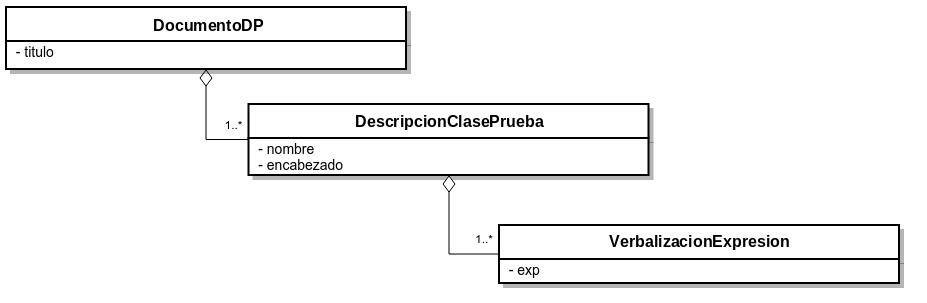
\includegraphics[scale=0.13]{img/document_plan.png}
  \end{figure}
\end{column}%
\end{columns}
\end{frame}
                                
\begin{frame}{Determinación de contenido}{}
  Esta tarea involucra uno o más procesos de \textbf{selección} y \textbf{razonamiento con los datos}.
  \begin{itemize}
    \item Nuestra tarea de \textbf{selección} debe, básicamente, buscar e incluir en el \textit{document plan} la o las clases de prueba a describir.
    \item Nuestras tareas de \textbf{razonamiento con los datos} como la eliminación de tautologías y la reducción de expresiones mejoran sustancialmente la calidad de los textos generados por nuestro sistema.
  \end{itemize}
\end{frame}
                                
\begin{frame}{Razonamiento con los datos}{Eliminación de tautologías}
  La \textbf{eliminación de tautologías} se encarga de filtrar expresiones que no añaden información adicional a las descripciones.
  \begin{figure}[H]
    \centering
    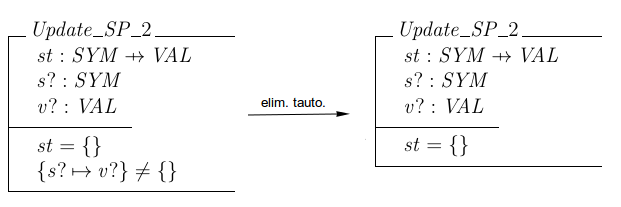
\includegraphics[scale=0.4]{img/ej_elim_tauto.png}
  \end{figure}
\end{frame}
                                
\begin{frame}{Razonamiento con los datos}{Reducción de expresiones}
  Reducir algunas expresiones nos permite simplificar las descripciones de las mismas.
  \begin{figure}[H]
    \centering
    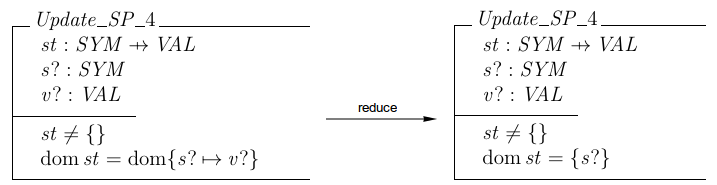
\includegraphics[scale=0.4]{img/ej_reduce.png}
  \end{figure}
\end{frame}
                                
\begin{frame}{Estructuración del documento}{}

  La \textbf{estructuración del documento} se ocupa de organizar y estructurar la información que el sistema debe comunicar. Por ejemplo, el \textit{document plan} para la descripción de \textit{LookUp\_SP\_1}:
  
  \begin{figure}[H]
    \centering
    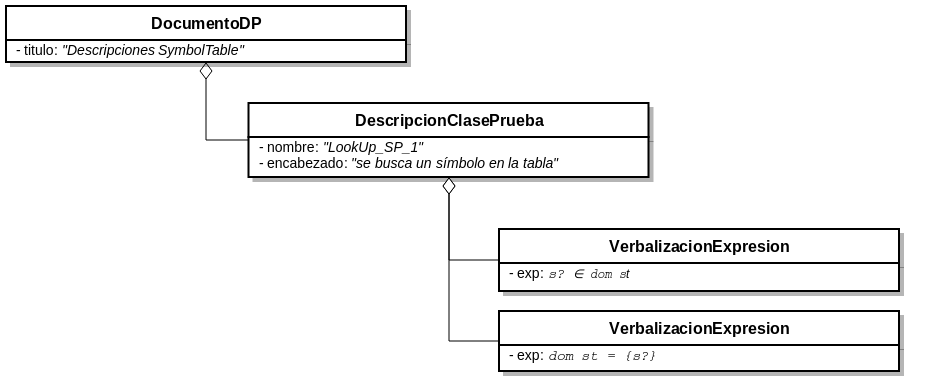
\includegraphics[scale=0.3]{img/document_plan_ej.png}
  \end{figure}
\end{frame}
                                
\subsection{Microplanning}

\begin{frame}{Microplanner}{}
  \begin{itemize}
    \item El módulo \textit{Microplanner} es el encargado de transformar el \textit{document plan} en una especificación más detallada del texto a generar.

    %\item La tarea más relevante que realiza este módulo en nuestro trabajo es la de \textit{lexicalización}.

    \item La tarea de \textbf{lexicalización}, será la principal tarea desarrollada en esta etapa y se encarga de elegir las palabras particulares y constructores sintácticos para comunicar la información contenida en el \textit{document plan}.

    \item Es en esta etapa donde hacemos uso de la información contenida en las designaciones.
  \end{itemize}
\end{frame}

\begin{frame}[fragile]{Microplanner}{Entrada y salida}
\begin{columns}[T] % align columns
\begin{column}{.50\textwidth}
  Entrada (\textit{document plan})
    \rule{\linewidth}{1pt}

  \begin{figure}[H]
    \centering
    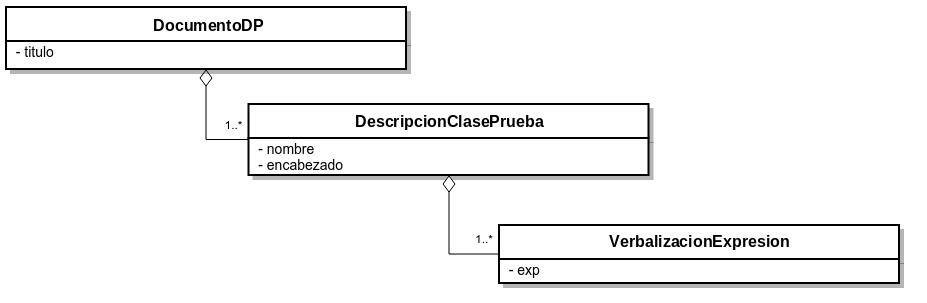
\includegraphics[scale=0.13]{img/document_plan.png}
  \end{figure}
\end{column}%
\hfill%
\begin{column}{.50\textwidth}
Salida (especificación del texto)
\rule{\linewidth}{1pt}

  \begin{figure}[H]
    \centering
    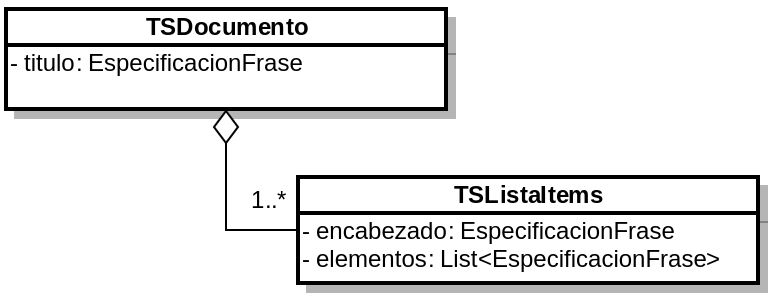
\includegraphics[scale=0.2]{img/text_spec.png}
  \end{figure}
\end{column}%
\end{columns}
\end{frame}
                                
\begin{frame}[fragile]{Lexicalización}{}

  Para esta tarea tenemos que tener en cuenta el conjunto de reglas para la verbalización de expresiones obtenidas durante el análisis del corpus.
  
  \begin{algorithm}[H]
    \caption{Bosquejo algoritmo lexicalización}
    \scriptsize
    \begin{algorithmic}[1]
    \Function {lexicalizacion}{exp}
    \If{\Call{esta\_designada}{exp}}
    \State ret $\gets$ \Call{designacion}{exp}
    \Else
    \State ret $\gets$ \Call{lexicalizacion'}{exp}
    \EndIf
    \State \textbf{return} ret
    \EndFunction
    \end{algorithmic}
  \end{algorithm}
\end{frame}

\begin{frame}[fragile]{Lexicalización}{Lexicalización operador $\in$}
  
  \begin{algorithm}[H]
    \caption{Caso de \textsc{lexicalizacion} del operador $\protect\in$}
    \scriptsize
    \begin{algorithmic}[1]
    \Function {lexicalizacion'}{x $\protect\in$ y}
    \State oracion.sujeto $\gets$ \Call{lexicalizacion}{x}
    \State fraseVerbal.verbo $\gets$ \text{\textit{``pertenecer''}}
    \State fraseEnlatada.texto $\gets$ \text{\textit{``a''}}
    \State elemYuxtapuesto.elementos $\gets$ \{fraseEnlatada, \Call{lexicalizacion}{y}\}
    \State fraseVerbal.complemento $\gets$ elemYuxtapuesto
    \State oracion.predicado $\gets$ fraseVerbal
    \State \textbf{return} oracion
    \EndFunction
    \end{algorithmic}
  \end{algorithm}

\end{frame}

\begin{frame}[fragile]{Lexicalización}{Ejemplo: especificación de frase para $s? \in \dom st$}
  
  \begin{figure}[H]
    \centering
    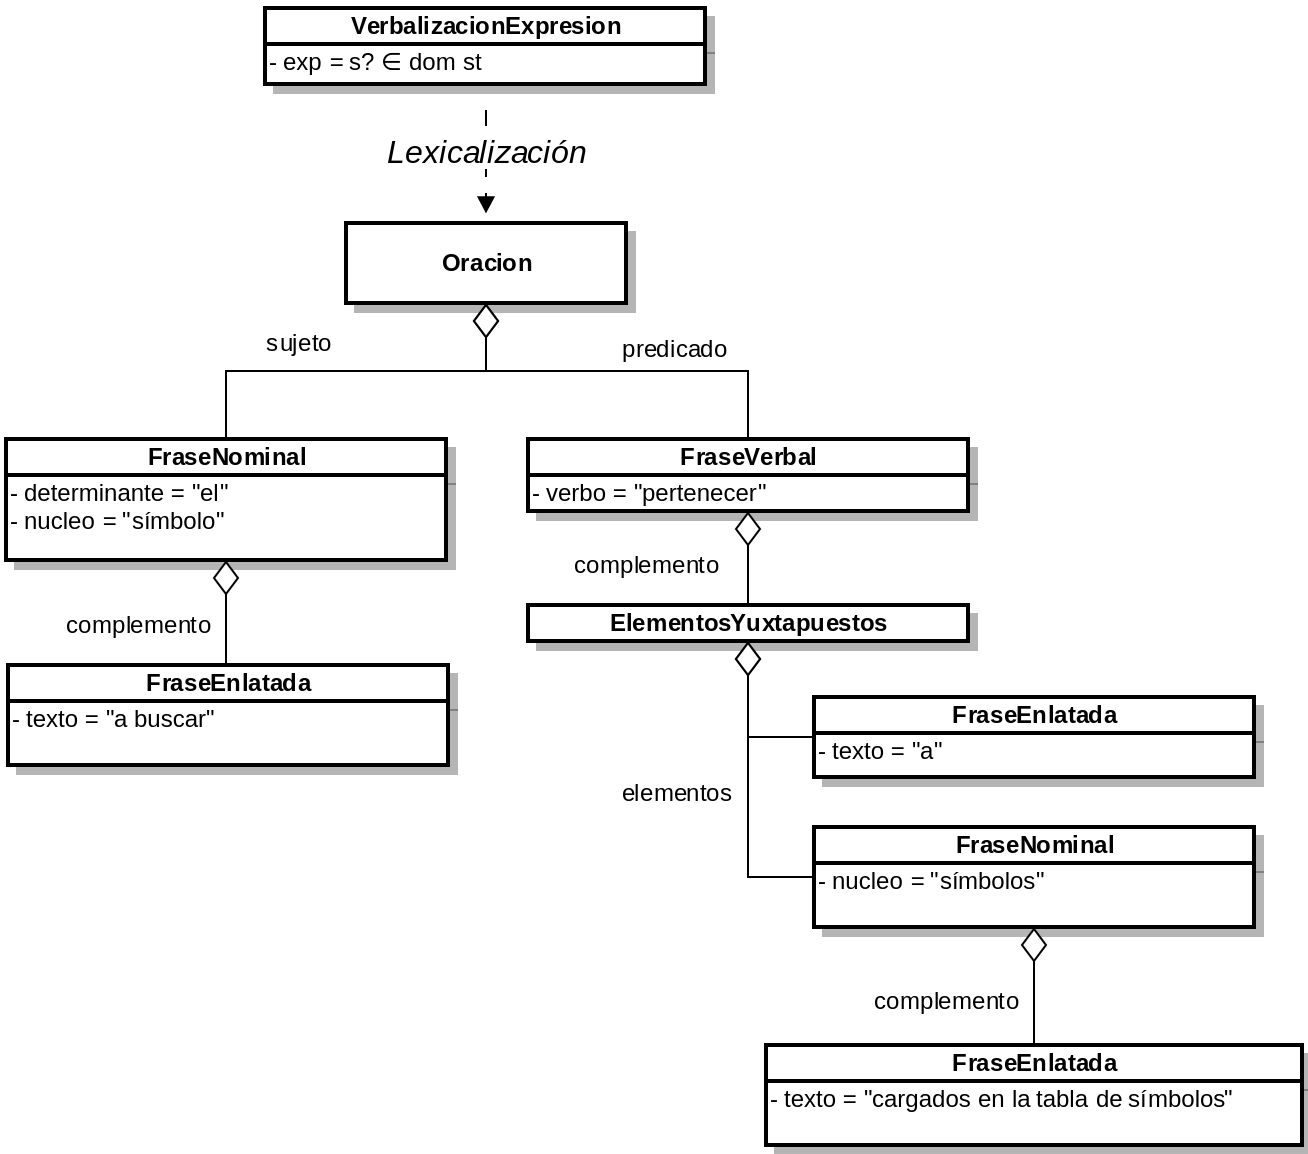
\includegraphics[scale=0.35]{img/phrase_spec_ej.png}
  \end{figure}

\end{frame}

\subsection{Surface Realization}

\begin{frame}{Surface Realizer}{}
  \begin{itemize}
    \item El módulo \emph{surface realizer} es el último del \emph{pipeline} de nuestro sistema NLG.

    \item El objetivo del mismo es transformar la especificación del texto en texto de superficie. 

    \item Este texto estará formado por anotaciones dependientes del sistema de presentación y oraciones generadas por la tarea de realización lingüística.

    %\item Éste tiene la misión de transformar la especificación de texto generada en la etapa anterior en texto de superficie, formado por frase, signos de puntuación y algunas anotaciones necesarias para el sistema de presentación utilizado (latex, html, etc).

    \item En la etapa de realización de superficie se llevarán a cabo dos tareas: \textbf{realización estructural} y \textbf{realización lingüística}.
  \end{itemize}
\end{frame}

\begin{frame}[fragile]{Ejemplo realización de superficie}{}
  Transformación llevada a cabo en esta etapa, para el ejemplo de \emph{LookUp\_SP\_1}:
  \begin{figure}[H]
    \centering
    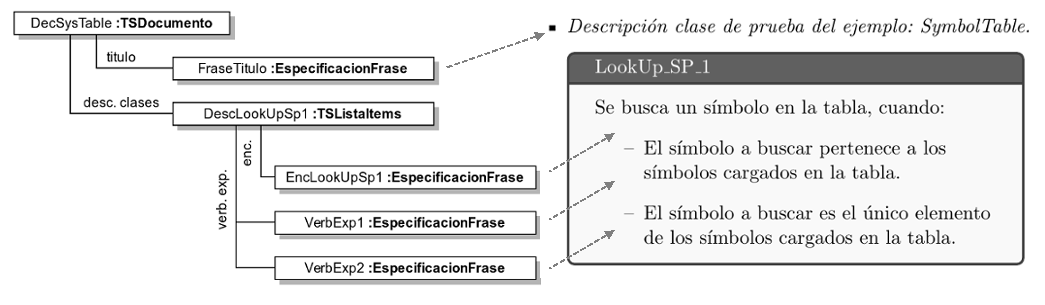
\includegraphics[scale=0.3]{img/ej_text_spec.png}
  \end{figure}
\end{frame}

\begin{frame}[fragile]{Surface Realizer}{Ejemplo salida}
  \begin{figure}[H]
  
  Texto resultado de la realización de superficie para \emph{LookUp\_SP\_1}:

  \begin{minted}
  [
  fontsize=\footnotesize,
  ]{latex}
  \documentclass{article}
  \title{Descripción clase de prueba del ejemplo: SymbolTable}
  \begin{document}
  \maketitle

  LookUp\_SP\_1: Se busca un símbolo en la tabla, cuando:
  \begin{itemize}
    \item El símbolo a buscar pertenece a los símbolos
      cargados en la tabla.
    \item El símbolo a buscar es el único elemento de los
      símbolos cargados en la tabla.  
  \end{itemize}
  
  \end{document}
  \end{minted}
  \end{figure}
\end{frame}
                                
\begin{frame}{Realización estructural}{}
  \begin{itemize}
    \item Es la tarea encargada de transformar los elementos de la especificación del texto en constructores del sistema de presentación.

    \item Para esto utiliza símbolos o etiquetas dependientes del sistema de presentación. Por ejemplo, las sentencias de \LaTeX{} necesarias para mostrar una lista de ítems.

    \item La realización estructural hace uso de las oraciones generadas por la tarea de \textbf{realización lingüística} fin de generar el texto final.
  \end{itemize}
\end{frame}

\begin{frame}[fragile]{Realización lingüística}{}
  \begin{itemize}
    \item Desempeña su tarea a nivel de la oración.

    \item La misión de la misma es transformar las especificaciones de frase en oraciones bien formadas.

    \item Entendiendo por oraciones bien formadas aquellas que cumplan con las reglas ortográficas y gramaticales del castellano (en nuestro caso).
    
    \item El realizador lingüístico debe tener en cuenta todos los requerimientos gramaticales obtenidos del corpus de descripciones.

  \end{itemize}
\end{frame}


\begin{frame}[fragile]{Realización lingüística}{}
  La tarea de realización lingüística es definida por casos para cada uno de los posibles elementos de una especificación de texto. Por ejemplo para realizar una Oración:

  \begin{algorithm}[H]
  \caption{Realización lingüística Oracion}
  \scriptsize
  \begin{algorithmic}[1]
  \Function {verbalizar}{Oracion oracion}
  \State sujeto $\gets$ \Call{verbalizar}{oracion.sujeto}
  \State fverbal $\gets$ oracion.predicado
  \State verbo $\gets$ \Call{determinar\_verbo}{fverbal.verbo, oracion.sujeto}
  \State atributo $\gets$ \Call{determinar\_atributo}{fverbal.atributo, oracion.sujeto}
  \State complemento $\gets$ \Call{verbalizar}{fverbal.complemento}
  \State resultado $\gets$ \Call{concat}{sujeto, verbo, atributo, complemento}
  \State \textbf{return} resultado
  \EndFunction
  \end{algorithmic}
  \end{algorithm}
\end{frame}
                                
\section{Conclusión y trabajos futuros}
\begin{frame}{Conclusión}{}

Conclusiones:
\begin{itemize}
  \item Pudimos desarrollar una solución para la generación automática de descripciones en lenguaje natural para clases de prueba generadas por el TTF.

  \item La solución propuesta es independiente del dominio de aplicación y del número de operaciones del sistema.

  \item Implementamos exitosamente un prototipo que fue integrado a las funcionalidades de Fastest.
\end{itemize}    
\end{frame}

\begin{frame}{Trabajo futuro}{}
Trabajos futuros:
\begin{itemize}
  \item Evaluación de textos generados por el sistema realizado (en términos de exactitud, fluidez, etc.).

  \item Ampliar la totalidad de operadores aceptados por el sistema.

  \item Profundizar el trabajo sobre los datos de entrada agregando más tareas de razonamiento con los datos.

  \item Expandir el sistema para que sea capaz de producir descripciones en otros idiomas.
\end{itemize}                         
\end{frame}
                                
% Section and subsections will appear in the presentation overview
% and table of contents.
%\section{First Main Section}
%                               
%\subsection{First Subsection}
%                               
%\begin{frame}{First Slide Title}{Optional Subtitle}
%  \begin{itemize}
%    \item      My first point.
%      }
%      \item        My second point.
%        }
%      \end{itemize}
%    \end{frame}
%                                                       
%    \subsection{Second Subsection}
%                                                       
%    % You can reveal the parts of a slide one at a time
%    % with the \pause command:
%    \begin{frame}{Second Slide Title}
%      \begin{itemize}
%        \item          First item.
%            \pause % The slide will pause after showing the first item
%          }
%          \item   
%              Second item.
%            }
%            % You can also specify when the content should appear
%            % by using <n->:
%            \item<3-> {
%              Third item.
%            }
%            \item<4-> {
%              Fourth item.
%            }
%            % or you can use the \uncover command to reveal general
%            % content (not just \items):
%            \item<5-> {
%              Fifth item. \uncover<6->{Extra text in the fifth item.}
%            }
%          \end{itemize}
%        \end{frame}
%                                                                               
%        \section{Second Main Section}
%                                                                               
%        \subsection{Another Subsection}
%                                                                               
%        \begin{frame}{Blocks}
%          \begin{block}{Block Title}
%            You can also highlight sections of your presentation in a block, with it's own title
%          \end{block}
%          \begin{theorem}
%            There are separate environments for theorems, examples, definitions and proofs.
%          \end{theorem}
%          \begin{example}
%            Here is an example of an example block.
%          \end{example}
%          \begin{beamercolorbox}[wd=7cm]{eecks}
%            asdasdasdsad
%          \end{beamercolorbox}
%        \end{frame}
%                                                                               
%        % Placing a * after \section means it will not show in the
%        % outline or table of contents.
%        \section*{Summary}
%                                                                               
%        \begin{frame}{Summary}
%          \begin{itemize}
%            \item
%              The \alert{first main message} of your talk in one or two lines.
%            \item
%              The \alert{second main message} of your talk in one or two lines.
%            \item
%              Perhaps a \alert{third message}, but not more than that.
%          \end{itemize}
%                                                                                           
%          \begin{itemize}
%            \item
%              Outlook
%              \begin{itemize}
%                \item
%                  Something you haven't solved.
%                \item
%                  Something else you haven't solved.
%              \end{itemize}
%          \end{itemize}
%        \end{frame}
%                                                                               
%                                                                               
%                                                                               
%        % All of the following is optional and typically not needed. 
%        \appendix
%        \section<presentation>*{\appendixname}
%        \subsection<presentation>*{For Further Reading}
%                                                                               
%        \begin{frame}[allowframebreaks]
%          \frametitle<presentation>{For Further Reading}
%                                                                                           
%          \begin{thebibliography}{10}
%                                                                                                       
%            \beamertemplatebookbibitems
%            % Start with overview books.
%                                                                                                       
%            \bibitem{Author1990}
%            A.~Author.
%            \newblock {\em Handbook of Everything}.
%            \newblock Some Press, 1990.
%                                                                                                       
%                                                                                                       
%            \beamertemplatearticlebibitems
%            % Followed by interesting articles. Keep the list short. 
%                                                                                                       
%            \bibitem{Someone2000}
%            S.~Someone.
%            \newblock On this and that.
%            \newblock {\em Journal of This and That}, 2(1):50--100,
%            2000.
%          \end{thebibliography}
%        \end{frame}
                                                                                      
\end{document} 
